\chapter{Implementación y despliegues}\label{ch:implementacion-y-despliegues}

En este capítulo se profundiza en los detalles de la implementación de la página web y la API a lo largo de los diferentes
\textit{sprints} que se han realizado durante el desarrollo del proyecto. Además, se explican los detalles de los despliegues
de la página web y la API así como las herramientas y tecnologías que se han utilizado para llevarlos a cabo.

\section{Desarrollo basado en sprints}\label{sec:desarrollo-basado-en-sprints}

Tal y como se ha mencionado en la subsección:~\ref{subsec:metodologia}, el desarrollo del proyecto se ha
realizado siguiendo una metodología ágil basada en \textit{sprints}. En este caso, se han ido completando los diferentes hitos del proyecto a lo largo de los
\textit{sprints} en los que se han incluidos tareas más específicas que permiten que el desarrollo sea más rápido y
eficiente.

\subsection{Sprints 1-4}\label{subsec:sprints-1-4}

En los cuatro primeros \textit{sprints} se han llevado a cabo las tareas que han permitido preparar los entornos de desarrollo
para la creación de la página web y la API. En concreto, se han llevado a cabo las siguientes tareas:

\begin{itemize}
    \item Creación de los repositorios de la página web y la API.
    \item Creación de la estructura de los proyectos y de la base de datos.
    \item Creación de la estructura inicial de la documentación del proyecto en \textit{LaTeX}.
    \item Fijación de objetivos y alcance del proyecto.
    \item Fijación de la metodología de desarrollo y requisitos del proyecto.
    \item Arquitectura del proyecto.
    \item Diseño de la API, página web y base de datos.
\end{itemize}

\subsubsection{Creación de la API}\label{subsubsec:creacion-de-la-api}

Para la creación de la API se ha usado el framework \textit{FastAPI} por medio del lenguaje de programación \textit{Python} el cual
se ha explicado en profundidad en la subsección:~\ref{subsec:framework-web-de-api}. Todo el código de la API se ha desarrollado
siguiendo la documentación oficial de \textit{FastAPI} que se puede consultar en la siguiente dirección: \url{https://fastapi.tiangolo.com/} y
las buenas prácticas de desarrollo de APIs que se pueden consultar en la siguiente dirección: \url{https://docs.microsoft.com/en-us/azure/architecture/best-practices/api-design}.
A continuación se van a mostrar los pasos que se han seguido en concreto para la creación de la API del proyecto:

\begin{enumerate}
    \item Instalar \textit{FastAPI} y \textit{uvicorn} por medio de \textit{pip} con el comando
    \textit{pip install fastapi uvicorn}.
    \item Crear un fichero \textit{main.py} que contendrá el código de la API que se ejecutará con el comando
    \textit{uvicorn main:app --reload}. El parámetro \textit{--reload} permite que cada vez que se realice un cambio
    en el código, el servidor se reinicie automáticamente.
    \item Definir las clases y esquemas de datos que se van a utilizar en la API.
    \item Definir las rutas que tendrá la API. En este proyecto se han definido las siguientes:
        \begin{itemize}
            \item \textbf{/auth}: ruta para reestablecer la contraseña de un usuario u organización
            \item \textbf{/organizations}: ruta que engloba todos los endpoints relacionados con las organizaciones
            \item \textbf{/users}: ruta que engloba todos los endpoints relacionados con los usuarios
            \item \textbf{/animals}: ruta que engloba todos los endpoints relacionados con los animales
            \item \textbf{/petitions}: ruta que engloba todos los endpoints relacionados con las peticiones
            \item \textbf{/filters}: ruta que engloba todos los endpoints relacionados con los filtros de búsqueda
        \end{itemize}
    \item Implementar los diferentes \textit{endpoints} dentro de cada ruta.
    \item Crear los tests para cada uno de los \textit{endpoints} de la API. Estos tests se pueden consultar en la
    subsección de testing:~\ref{subsubsec:tests}.
\end{enumerate}

\subsubsection{Clases}\label{subsubsec:clases}

Antes de iniciar con la implementación de los \textit{endpoints} de la API es necesario definir las clases y esquemas de datos
que se van a utilizar. En la siguiente imagen se puede ver de forma esquemática las clases que se han definido para el proyecto:

\begin{figure}[H]
    \centering
    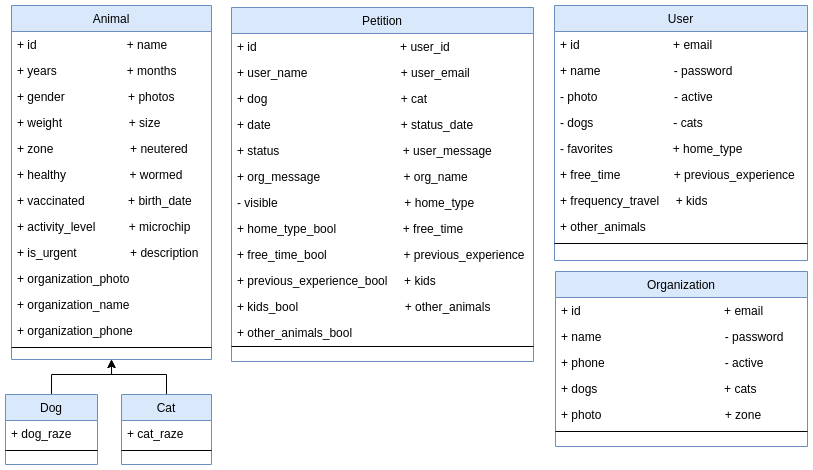
\includegraphics[width=0.9\textwidth]{imgs/clases.png}
    \caption{Clases}
    \label{fig:clases}
\end{figure}

Como vemos se han definido las siguientes clases:

\begin{itemize}
    \item \textbf{Animal}: con sus respectivos atributos (id, años, nombre, fotos, etc.)
    \item \textbf{Dog}: que hereda de la clase \textit{Animal} y que añade su propio atributo (raza)
    \item \textbf{Cat}: que hereda de la clase \textit{Animal} y que añade su propio atributo (raza)
    \item \textbf{Petition}: con sus respectivos atributos (id, fecha, estado, etc.)
    \item \textbf{User}: con sus respectivos atributos (id, nombre, foto, etc.)
    \item \textbf{Organization}: con sus respectivos atributos (id, nombre, email, foto, etc.)
\end{itemize}

Además se ha diferenciado si el atributo es de consulta \textbf{privado} por medio del símbolo \textit{-} o de consulta
\textbf{público} por medio del símbolo \textit{+}. Por ejemplo, el atributo \textit{email} de la clase \textit{Organization}
es público porque se puede consultar por medio de la API, mientras que el atributo \textit{password} de la clase
\textit{User} es privado ya que no sería recomendable que se pudiera acceder a él por medio de una consulta.

\subsubsection{Códigos de estado de respuesta HTTP}\label{subsubsec:codigos-de-error}

A la hora de implementar una API, es importante tener en cuenta los códigos de estado que se pueden devolver en cada petición HTTP. En este caso, se ha
seguido la especificación de \href{https://developer.mozilla.org/es/docs/Web/HTTP/Status}{MDN Web Docs} para devolver los códigos más
adecuados en cada caso. A continuación, se muestra una tabla con los diferentes códigos que se han utilizado a lo largo del desarrollo:

\begin{table}[H]
    \centering
    \begin{tabular}{|c|c|}
        \hline
        \textbf{Código de error} & \textbf{Descripción} \\
        \hline
        200 & OK \\
        \hline
        204 & Sin contenido \\
        \hline
        400 & Petición incorrecta \\
        \hline
        401 & No autorizado \\
        \hline
        403 & Prohibido \\
        \hline
        404 & No encontrado \\
        \hline
        500 & Error interno del servidor \\
        \hline
    \end{tabular}
    \caption{Códigos de respuesta HTTP}
    \label{tab:codigos-respuesta-http}
\end{table}

Un ejemplo de ello podría ser la petición de adopción de una mascota. Si el usuario no está autenticado en el sistema, se devolvería un código de error
401 (no autorizado). Si el usuario está autenticado, pero no se ha encontrado la mascota que se quiere adoptar, se devolvería un código de error 404 (no encontrado).
Si la petición se ha realizado correctamente, se devolvería un código de estado 200 (OK). \\

Los códigos de error 500 (error interno del servidor) y 400 (petición incorrecta) se han utilizado en casos en los que se ha producido un error en el servidor
o en el cliente, respectivamente. Por ejemplo, si se ha producido un error al realizar una consulta a la base de datos, se devolvería un código de error 500.
Si el usuario ha enviado una petición con un formato incorrecto, se devolvería un código de error 400.

\subsubsection{Creación de la página web}\label{subsubsec:creacion-de-la-pagina-web}

La estructura del proyecto en Angular se basa en componentes, servicios y módulos (patrón módulo). Los módulos se utilizan
para organizar y estructurar la aplicación en diferentes partes así como separar la lógica en diferentes ficheros. Cada módulo
se compone de componentes y servicios. Los componentes se encargan de la parte visual de la aplicación y los servicios
se encargan de la lógica de la aplicación. El proyecto de la página web se compone de los siguientes elementos:

\begin{itemize}
    \item \textbf{Directorio \textit{src}:} directorio principal de la aplicación. En este directorio se encuentran los ficheros
    de configuración de la aplicación, los ficheros de \textit{testing} y los ficheros de la aplicación. También se encuentran
    los componentes, servicios, directivas y el resto de elementos.
    \item \textbf{Directorio \textit{app}:} este directorio contiene el componente principal de la aplicación, el componente \textit{app.component}.
    Este es el componente que se carga al iniciar la aplicación y que a su vez contiene la llamada al resto de componentes.
    \item \textbf{Directorio \textit{assets}:} este directorio contiene los recursos de la aplicación como imágenes, iconos, etc.
    \item \textbf{Directorio \textit{environments}:} este directorio contiene los ficheros de configuración de los entornos de la aplicación (producción y desarrollo).
    \item \textbf{Directorio \textit{services}:} este directorio contiene los diferentes servicios de la aplicación que se encargan a su vez de realizar
    las peticiones a la API.
    \item \textbf{Directorio \textit{components}:} este directorio contiene los diferentes componentes de la aplicación. Cada componente se compone de un fichero
    \textit{.ts} que contiene la lógica del componente, un fichero \textit{.html} que contiene la parte visual del componente, un fichero \textit{.scss}
    que contiene los estilos del componente y un fichero \textit{.spec.ts} que contiene los tests del componente.
    \item \textbf{Directorio \textit{interfaces}:} este directorio contiene las interfaces de la aplicación. Estas interfaces se utilizan para definir
    los tipos de datos que se van a utilizar en la aplicación.
    \item \textbf{Archivo \textit{index.html}:} este archivo contiene la estructura básica de la página web. Aquí se vinculan los diferentes ficheros de estilos
    y scripts necesarios para el correcto funcionamiento de la aplicación.
\end{itemize}

Esta estructura ofrece numerosas ventajas frente a otros \textit{frameworks} como puede ser la \textbf{modularidad} de la aplicación. De esta forma,
la aplicación se convierte más fácil de mantener y de escalar. Otra de las ventajas es la \textbf{reutilización} de componentes. De esta forma, si
se quiere utilizar un componente en diferentes partes de la aplicación, solo es necesario importarlo en el componente que se desee. También
ofrece la ventaja de la \textbf{separación de responsabilidades}. Existen servicios, componentes, directivas y otros elementos
que de forma individual se encargan de una tarea concreta.

\subsubsection{Creación de Bases de Datos}\label{subsec:creacion-de-bases-de-datos}

Para el proyecto se han creados dos bases de datos: una para la versión de desarrollo y otra para la versión de producción.
Ambas, por medio de \textbf{Firebase} cuentan con la misma estructura y se encuentran en la nube, pero la base de datos de
producción cuenta con una serie de reglas que limitan el acceso a la misma y que se detallan en la subsección:~\ref{subsubsec:reglas} a
diferencia de la base de datos de desarrollo que no cuenta con ese tipo de restricciones y que se ha usado exclusivamente para
probar la funcionalidad de la API. \\

Las bases de datos de Firebase son bases de datos no relacionales que se basan en colecciones que pueden contener un número ilimitado de documentos.
Cada documento a su vez se compone de una serie de campos que pueden ser de diferentes tipos (texto, número, booleano, etc.).
Vamos a desgranar cada uno de estos conceptos en las siguientes subsecciones.

\newpage

\subsubsection{Colecciones}\label{subsubsec:colecciones}

Las colecciones son el elemento principal de las bases de datos de Firebase. Cada colección puede contener un número ilimitado de documentos
y cada documento puede contener un número ilimitado de campos. Podemos ver las colecciones como las tablas de una base de datos relacional
y los documentos como las filas de dichas tablas. \\

En este proyecto se han creado las siguientes colecciones:

\begin{itemize}
    \item \textbf{Animals}: Colección que contiene un documento \textit{animals} que a su vez contiene todos los animales que se encuentran en la base de datos.
    \item \textbf{Users}: Colección que contiene un documento con el \textit{id} de cada usuario que se ha registrado en la aplicación y que a su vez contiene
    todos los datos de dicho usuario.
    \item \textbf{Organization}: Colección que contiene un documento con el \textit{id} de cada organización que se ha registrado en la aplicación y que a su vez contiene
    todos los datos de dicha organización.
    \item \textbf{Petitions}: Colección que contiene un documento con el \textit{id} de cada petición que se ha realizado en la aplicación y que a su vez contiene
    todos los datos de dicha petición.
\end{itemize}

En la siguiente figura se puede ver un ejemplo de la estructura de la base de datos de desarrollo: \\

\begin{figure}[H]
    \centering
    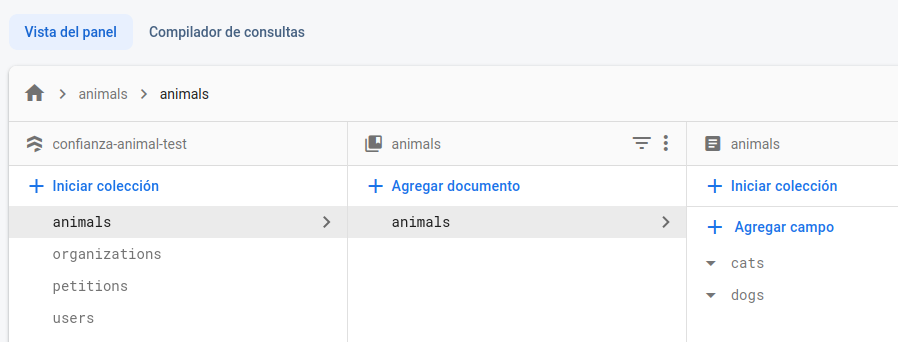
\includegraphics[width=0.9\textwidth]{imgs/database-test.png}
    \caption{Ejemplo de estructura de la base de datos de desarrollo}
    \label{fig:database}
\end{figure}

\newpage

\subsubsection{Datos}\label{subsubsec:datos}

Firebase cuenta con una gran variedad de tipos de datos que se pueden utilizar para almacenar información en la base de datos.
A parte de los tipos de datos básicos como texto, número o booleano, Firebase cuenta con tipos de datos más complejos como
imágenes y archivos que se han utilizado para almacenar las imágenes de los animales, usuarios y organizaciones,
datos de geolocalización en tiempo real o fechas y horas. \\

En este proyecto se han utilizado todo tipo de datos para almacenar la información de los animales, usuarios y organizaciones.
Por ejemplo, para almacenar la información de un animal se ha utilizado el siguiente formato:

\begin{table}[H]
\begin{tabular}{ll}
\textit{\textbf{Variable}} & \textit{\textbf{Tipo de dato}} \\
Nombre                     & \textit{string}                \\
Años                       & \textit{int}                   \\
Meses                      & \textit{int}                   \\
Género                     & \textit{string}                \\
Fotos                      & \textit{photo{[}{]}}             \\
Peso                       & \textit{float}                 \\
Tamaño                     & \textit{string}                \\
Provincia                  & \textit{string}                \\
Castrado                   & \textit{booleano}              \\
Sano                       & \textit{booleano}              \\
Vacunado                   & \textit{booleano}              \\
Fecha de nacimiento        & \textit{datetime}              \\
Microchip                  & \textit{booleano}              \\
Actividad                  & \textit{string}                \\
Urgente                    & \textit{booleano}              \\
Raza                       & \textit{string}                \\
Descripción                & \textit{string}
\end{tabular}
\end{table}

\newpage

\subsubsection{Reglas}\label{subsubsec:reglas}

El sistema de reglas de \textbf{Firebase} son una parte fundamental para la seguridad de la base de datos. Estas reglas
permiten limitar el acceso a la base de datos a usuarios que cumplan una serie de condiciones y se basan en el
lenguaje de expresiones de \textbf{Firebase} (\textit{Firebase's expression language}) que se configuran en
el archivo \textit{firestore.rules} que se encuentra en la raíz del proyecto. \\

Existen dos tipos de reglas: las reglas de validación y las reglas de seguridad. La primera de ellas se encarga de
validar los datos que se van a almacenar en la base de datos y la segunda se encarga de limitar el acceso a la base de datos.
En nuestro caso, como las validaciones se realizan en el \textit{backend} de la aplicación, las reglas de validación
se han dejado vacías y las reglas de seguridad se han configurado en función del entorno de la aplicación. \\

Para la base de datos de desarrollo se quiere que cualquier usuario pueda acceder a la misma, por lo que las reglas
de seguridad permiten el acceso de lectura y escritura a cualquier usuario autenticado:

\begin{lstlisting}
{
    "rules": {
    ".read": "request.auth != null",
    ".write": "request.auth != null"
    }
}
\end{lstlisting}

Para la base de datos de producción las reglas son más estrictas para proteger la información de los usuarios.
De esta forma, solo se permite el acceso a usuarios autenticados y se limita el acceso a la base de datos
en función del tipo de usuario que se haya autenticado y de la colección a la que quiera acceder. Por ejemplo, un usuario normal
puede escribir y leer en su colección de usuario pero no puede escribir en la colección de organizaciones.:

\newpage

\begin{lstlisting}
{
"rules": {
        "Animals": {
            ".read": "request.auth != null",
            ".write": "request.auth != null"
        },
        "Users": {
            "$uid": {
                ".read": "request.auth != null",
                ".write": "request.auth != null && request.auth.uid == $uid"
            }
        },
        "Organization": {
            "$uid": {
                ".read": "request.auth != null",
                ".write": "request.auth != null && request.auth.uid == $uid"
            }
        },
        "Petitions": {
            ".read": "request.auth != null",
            ".write": "request.auth != null"
        }
    }
}

\end{lstlisting}



\subsection{Sprints 5-8}\label{subsec:sprints-5-8}

Una vez que se han completado las tareas que permiten el desarrollo e implementación de la página web y la API, durante los
cuatro siguientes \textit{sprints} se han llevado a cabo las tareas que han permitido la implementación de la página web y la API
así como la realización de los tests y despliegues de ambas:

\begin{itemize}
    \item Creación de \textit{endpoints} para la API.
    \item Creación de componentes para la página web.
    \item Creación de servicios para la página web.
    \item Creación de \textit{tests} para la API y la página web.
\end{itemize}

\subsubsection{Endpoints}\label{subsubsec:endpoints}

Una vez que se ha definido la estructura de la API y conocemos las diferentes clases que se van a utilizar, podemos
pasar a definir e implementar los diferentes \textit{endpoints} para cumplir con los requisitos de la API.\\

Un \textit{endpoint} es un punto de entrada de la API que permite realizar una acción concreta. Es decir,
se refiere a la ruta que se va a utilizar para acceder a un recurso concreto. Por ejemplo, si queremos acceder a la
información de un usuario concreto, la ruta que se utilizaría sería \textit{/users/{user\_id}} siendo \textit{use\_id}
el identificador del usuario. A continuación se van a mostrar los diferentes \textit{endpoints} que se han definido para
el proyecto: \\

\textbf{Ruta:} \textit{/auth}

\begin{itemize}
    \item \textbf{/reset-password}: \textit{POST} \\
    Permite reestablecer la contraseña de un usuario u organización por medio de un correo electrónico que se envía
    a la dirección de correo electrónico registrada en el sistema.
\end{itemize}

\textbf{Ruta:} \textit{/organizations}

\begin{itemize}
    \item \textbf{/me}: \textit{GET} \\
    Permite obtener toda la información de la organización que ha iniciado sesión en el sistema (correo, nombre, foto, etc.).
    \item \textbf{/dogs}: \textit{GET} \\
    Permite obtener todos los perros de la organización que ha iniciado sesión en el sistema en forma de lista.
    \item \textbf{/cats}: \textit{GET} \\
    Permite obtener todos los gatos de la organización que ha iniciado sesión en el sistema en forma de lista.
    \item \textbf{/}: \textit{GET} \\
    Permite obtener una información reducida de todas las organizaciones registradas en el sistema: nombre, correo, foto y provincia.
    \item \textbf{/{organization\_name}}: \textit{GET} \\
    Dado un nombre de organización existente en el sistema, permite obtener toda la información de la organización: nombre, correo, foto, provincia, etc.
    \item \textbf{/dog}: \textit{POST} \\
    Permite crear un nuevo perro en la organización que ha iniciado sesión en el sistema pasando como parámetros los atributos del perro.
    \item \textbf{/cat}: \textit{POST} \\
    Permite crear un nuevo gato en la organización que ha iniciado sesión en el sistema pasando como parámetros los atributos del gato.
    \item \textbf{/register}: \textit{POST} \\
    Permite registrar una nueva organización en el sistema pasando como parámetros los atributos de la organización: nombre, correo, contraseña, teléfono y provincia.
    \item \textbf{/login}: \textit{POST} \\
    Permite iniciar sesión en el sistema pasando como parámetros el correo y la contraseña de la organización.
    \item \textbf{/upload/photo}: \textit{POST} \\
    Permite subir una foto de perfil para la organización que ha iniciado sesión en el sistema.
    \item \textbf{/enable}: \textit{POST} \\
    Permite activar la cuenta de la organización que ha iniciado sesión en el sistema siempre y cuando haya sido desactivada previamente.
    \item \textbf{/dog/{dog\_id}}: \textit{PUT} \\
    Permite modificar los atributos de un perro de la organización que ha iniciado sesión en el sistema pasando como parámetros los atributos del perro.
    \item \textbf{/cat/{cat\_id}}: \textit{PUT} \\
    Permite modificar los atributos de un gato de la organización que ha iniciado sesión en el sistema pasando como parámetros los atributos del gato.
    \item \textbf{/update}: \textit{PUT} \\
    Permite modificar los atributos de la organización que ha iniciado sesión en el sistema pasando como parámetros los atributos a actualizar: teléfono y provincia.
    \item \textbf{/disable}: \textit{DELETE} \\
    Permite desactivar la cuenta de la organización que ha iniciado sesión en el sistema. Una vez desactivada, la organización no podrá iniciar sesión en el sistema.
\end{itemize}

\textbf{Ruta:} \textit{/users}

\begin{itemize}
    \item \textbf{/me}: \textit{GET} \\
    Permite obtener toda la información del usuario que ha iniciado sesión en el sistema (correo, nombre, foto, etc.).
    \item \textbf{/favorites}: \textit{GET} \\
    Permite obtener todos los perros y gatos favoritos del usuario que ha iniciado sesión en el sistema en forma de lista.
    \item \textbf{/favorites/{animal\_id}}: \textit{GET} \\
    Dado un identificador de perro o gato, devuelve si el animal es favorito del usuario que ha iniciado sesión en el sistema.
    \item \textbf{/{user\_id}}: \textit{GET} \\
    Dado un identificador de usuario, permite obtener toda la información del usuario: nombre, correo, foto, etc.
    \item \textbf{/favorites/{animal\_id}}: \textit{POST} \\
    Permite añadir un perro o gato a la lista de favoritos del usuario que ha iniciado sesión en el sistema.
    \item \textbf{/update}: \textit{PUT} \\
    Permite modificar los atributos del usuario que ha iniciado sesión en el sistema pasando como parámetros los atributos a actualizar: nombre, teléfono, provincia...
    \item \textbf{/documentation/{petition\_id}}: \textit{POST} \\
    Permite al usuario simular el envío de documentación a la organización dado un identificador de petición de adopción.
    \item \textbf{/register}: \textit{POST} \\
    Permite registrar un nuevo usuario en el sistema pasando como parámetros los atributos del usuario: correo, nombre y contraseña.
    \item \textbf{/login}: \textit{POST} \\
    Permite iniciar sesión en el sistema pasando como parámetros el correo y la contraseña del usuario.
    \item \textbf{/enable}: \textit{POST} \\
    Permite activar la cuenta del usuario que ha iniciado sesión en el sistema siempre y cuando haya sido desactivada previamente.
    \item \textbf{/upload/photo}: \textit{POST} \\
    Permite subir una foto de perfil para el usuario que ha iniciado sesión en el sistema.
    \item \textbf{/update-documentation/{petition\_id}}: \textit{POST} \\
    Permite al usuario simular la actualización de la documentación de una petición de adopción dado un identificador de petición de adopción
    siempre y cuando la misma haya sido rechazada por la organización previamente.
    \item \textbf{/disable}: \textit{DELETE} \\
    Permite desactivar la cuenta del usuario que ha iniciado sesión en el sistema. Una vez desactivada, el usuario no podrá iniciar sesión en el sistema.
    \item \textbf{/favorites/{animal\_id}}: \textit{DELETE} \\
    Permite eliminar un perro o gato de la lista de favoritos del usuario que ha iniciado sesión en el sistema.
\end{itemize}

\textbf{Ruta:} \textit{/animals}

\begin{itemize}
    \item \textbf{/}: \textit{GET} \\
    Permite obtener todos los perros y gatos registrados en el sistema en forma de lista.
    \item \textbf{/dog/{dog\_id}}: \textit{GET} \\
    Dado un identificador de perro, permite obtener toda la información del perro: nombre, edad, raza, etc.
    \item \textbf{/cat/{cat\_id}}: \textit{GET} \\
    Dado un identificador de gato, permite obtener toda la información del gato: nombre, edad, raza, etc.
    \item \textbf{/dog}: \textit{GET} \\
    Permite obtener todos los perros registrados en el sistema en forma de lista por medio de filtros que se pueden combinar entre sí:
        \begin{itemize}
            \item \textbf{\textit{province}}: Permite filtrar los perros por provincia.
            \item \textbf{\textit{size}}: Permite filtrar los perros por tamaño: mini, pequeño, mediano, grande o gigante.
            \item \textbf{\textit{raze}}: Permite filtrar los perros por raza.
            \item \textbf{\textit{years}}: Permite filtrar los perros por edad numérica.
            \item \textbf{\textit{greater\_or\_equal}}: Booleano que permite filtrar los perros por edad numérica mayor o igual que la especificada en el filtro anterior (\textit{years}).
            \item \textbf{\textit{gender}}: Permite filtrar los perros por género: macho o hembra.
            \item \textbf{\textit{activity}}: Permite filtrar los perros por nivel de actividad: bajo, medio o alto.
            \item \textbf{\textit{is\_urgent}}: Booleano que permite filtrar los perros en caso de ser su adopción urgente o no.
        \end{itemize}
    \item \textbf{/cat}: \textit{GET} \\
    Permite obtener todos los gatos registrados en el sistema en forma de lista por medio de los mismo filtros mencionados anteriormente para el caso de los perros.
    \item \textbf{/dog/{dog\_id}/photos}: \textit{POST} \\
    Permite subir una o varias fotos para un perro dado su identificador.
    \item \textbf{/cat/{cat\_id}/photos}: \textit{POST} \\
    Permite subir una o varias fotos para un gato dado su identificador.
    \item \textbf{/dog/{dog\_id}}: \textit{DELETE} \\
    Permite eliminar un perro del sistema dado su identificador. Sólo válido para organizaciones que además tengan ese animal en su lista.
    \item \textbf{/cat/{cat\_id}}: \textit{DELETE} \\
    Permite eliminar un gato del sistema dado su identificador. Sólo válido para organizaciones que además tengan ese animal en su lista.
    \item \textbf{/dog/{dog\_id}/photo}: \textit{DELETE} \\
    Permite eliminar una foto de un perro dado su identificador y el identificador de la foto.
    \item \textbf{/cat/{cat\_id}/photo}: \textit{DELETE} \\
    Permite eliminar una foto de un gato dado su identificador y el identificador de la foto.
\end{itemize}


\textbf{Ruta:} \textit{/petitions}

\begin{itemize}
    \item \textbf{/user}: \textit{GET} \\
    Permite obtener todas las peticiones de adopción realizadas por el usuario que ha iniciado sesión en el sistema.
    \item \textbf{/{petition\_id}/user}: \textit{GET} \\
    Permite obtener la información de una petición de adopción dado su identificador al usuario que ha iniciado sesión en el sistema.
    \item \textbf{/user/visibles}: \textit{GET} \\
    Permite obtener todas las peticiones de adopción visibles realizadas por el usuario que ha iniciado sesión en el sistema.
    \item \textbf{/user/invisibles}: \textit{GET} \\
    Permite obtener todas las peticiones de adopción invisibles realizadas por el usuario que ha iniciado sesión en el sistema.
    \item \textbf{/organization}: \textit{GET} \\
    Permite obtener todas las peticiones de adopción realizadas a la organización que ha iniciado sesión en el sistema.
    \item \textbf{/dog/{dog\_id}}: \textit{POST} \\
    Permite realizar una petición de adopción para un perro dado su identificador.
    \item \textbf{/cat/{cat\_id}}: \textit{POST} \\
    Permite realizar una petición de adopción para un gato dado su identificador.
    \item \textbf{/{petition\_id}/user}: \textit{POST} \\
    Permite cambiar la visibilidad de una petición de adopción dado su identificador al usuario que ha iniciado sesión en el sistema (visible o invisible).
    \item \textbf{/organization/{petition\_id}}: \textit{POST} \\
    Permite cambiar el estado de una petición de adopción dado su identificador a la organización que ha iniciado sesión en el sistema. El flujo de estados
    se puede ver en la figura~\ref{fig:flujo-peticion}.
    \item \textbf{/{petition\_id}/organization/documentation}: \textit{POST} \\
    Permite actualizar el estado de la petición una vez que el usuario ha subido la documentación requerida para la adopción por parte de la organización.
    \item \textbf{/{petition\_id}/organization/accept-information}: \textit{POST} \\
    Permite actualizar el estado de la petición para indicar que la organización ha aceptado la información aportada por el usuario para una petición de adopción concreta.
    \item \textbf{/{petition\_id}/organization/reject-information}: \textit{POST} \\
    Permite actualizar el estado de la petición para indicar que la organización ha rechazado la información aportada por el usuario para una petición de adopción concreta.
    \item \textbf{/{petition\_id}/organization}: \textit{POST} \\
    Permite actualizar el estado de la petición para indicar que la organización ha aceptado la petición de adopción por parte del usuario.
    \item \textbf{/{petition\_id}/user}: \textit{DELETE} \\
    Permite actualizar el estado de la petición a rechazada por parte del usuario.
    \item \textbf{/{petition\_id}/organization}: \textit{DELETE} \\
    Permite actualizar el estado de la petición a rechazada por parte de la organización.
\end{itemize}

\newpage

\textbf{Ruta:} \textit{/filters}

\begin{itemize}
    \item \textbf{/provinces}: \textit{GET} \\
    Permite obtener todas las provincias que se encuentran en el sistema (Madrid, Barcelona, etc.)
    \item \textbf{/gender}: \textit{GET} \\
    Permite obtener todos los géneros que se encuentran en el sistema (macho, hembra).
    \item \textbf{/activity}: \textit{GET} \\
    Permite obtener todas las actividades que se encuentran en el sistema (baja, media, alta).
    \item \textbf{/size}: \textit{GET} \\
    Permite obtener todos los tamaños que se encuentran en el sistema (pequeño, mediano, grande, etc.)
    \item \textbf{/cat-raze}: \textit{GET} \\
    Permite obtener todas las razas de gatos que se encuentran en el sistema (siamés, persa, etc.)
    \item \textbf{/dog-raze}: \textit{GET} \\
    Permite obtener todas las razas de perros que se encuentran en el sistema (pastor alemán, labrador, etc.)
    \item \textbf{/all}: \textit{GET} \\
    Permite obtener todos los filtros que se encuentran en el sistema (todos los anteriores).
\end{itemize}

\newpage

\subsubsection{Componentes}\label{subsubsec:componentes}

Si ponemos el ejemplo y pensamos que una aplicación web es una casa, los componentes serían las diferentes habitaciones de la casa. Cada componente
se encarga de una tarea concreta y se puede reutilizar en diferentes partes de la aplicación. A su vez, están formados por un fichero \textit{.ts}
que contiene la lógica del componente, un fichero \textit{.html} que contiene la parte visual del componente, un fichero \textit{.scss}
que contiene los estilos del componente y un fichero \textit{.spec.ts} que contiene los tests del componente. \\

Para diferenciar los componentes, en Angular son clases TypeScript decoradas con el decorador \textit{@Component}. Este decorador
es el que define los metadatos del componente como el selector, la plantilla, los estilos, etc. Un ejemplo de componente sería el siguiente:

\begin{lstlisting}
import { Component, OnInit } from '@angular/core';

@Component({
  selector: 'app-home',
  templateUrl: './home.component.html',
  styleUrls: ['./home.component.scss']
})

export class HomeComponent implements OnInit {

  constructor() { }

  ngOnInit(): void {
  }

}
\end{lstlisting}

En este ejemplo se puede observar que el componente se define con el decorador \textit{@Component} y que se le pasan los metadatos
correspondientes. En este caso, el selector del componente es \textit{app-home} y la plantilla y los estilos se encuentran en los ficheros
\textit{home.component.html} y \textit{home.component.scss} respectivamente. \\

Para utilizar un componente en otro, solo es necesario importarlo en la plantilla del componente que se desee. Por ejemplo, si se quiere
utilizar el componente \textit{home} en el componente \textit{app.component}, solo es necesario importarlo en la plantilla del componente
\textit{app.component} de la siguiente forma:

\begin{lstlisting}
<app-home></app-home>
\end{lstlisting}

En el proyecto de la página web se han utilizado los siguientes componentes:

\begin{itemize}
    \item \textbf{app.component}: este componente es el componente principal de la aplicación. Este componente se carga al iniciar la aplicación
    y contiene la llamada al resto de componentes.
    \item \textbf{home.component}: este componente es el componente que se carga al iniciar la aplicación. Este componente contiene la página principal
    de la aplicación.
    \item \textbf{login.component}: este componente contiene la página de inicio de sesión de la aplicación.
    \item \textbf{register.component}: este componente contiene la página de registro de la aplicación.
    \item \textbf{profile.component}: este componente contiene la página de perfil de la aplicación.
    \item \textbf{restore-password.component}: este componente contiene la página de recuperación de contraseña de la aplicación.
    \item \textbf{animals.component}: este componente contiene la página de animales de la aplicación.
    \item \textbf{cat-profile.component}: este componente contiene la página de perfil de un gato de la aplicación.
    \item \textbf{dog-profile.component}: este componente contiene la página de perfil de un perro de la aplicación.
    \item \textbf{cat-view.component}: este componente contiene la página de visualización de un gato de la aplicación.
    \item \textbf{dog-view.component}: este componente contiene la página de visualización de un perro de la aplicación.
    \item \textbf{new-animal.component}: este componente contiene la página de creación de un animal de la aplicación.
\end{itemize}

\newpage

\subsubsection{Servicios}\label{subsubsec:servicios}

Los servicios son clases que se utilizan para organizar y compartir métodos y datos entre diferentes componentes de la aplicación. Estos servicios
se pueden inyectar en los componentes que se deseen y suelen utilizarse para realizar peticiones HTTP a la API.
Para crear un servicio, en Angular se utiliza el decorador \textit{@Injectable}. Este decorador
es el que define los metadatos del servicio como el nombre del servicio, los servicios que se van a inyectar en el servicio, etc. Un ejemplo de servicio
sería el siguiente:

\begin{lstlisting}
import { Injectable } from '@angular/core';

@Injectable({
  providedIn: 'root'
})

export class AuthService {

  constructor() { }
}
\end{lstlisting}

En este ejemplo se puede observar que el servicio se define con el decorador \textit{@Injectable} y que se le pasan los metadatos
correspondientes. En este caso, el servicio se inyecta en el \textit{root} de la aplicación. Los servicios que se han utilizado en el proyecto
de la página web son los siguientes:

\begin{itemize}
    \item \textbf{auth.service}: este servicio se utiliza para realizar las peticiones HTTP relacionadas con la autenticación de la aplicación (inicio de sesión, registro, etc.)
    \item \textbf{user.service}: este servicio se utiliza para realizar las peticiones HTTP relacionadas con los usuarios (organizaciones) de la aplicación.
    \item \textbf{animals.service}: este servicio se utiliza para realizar las peticiones HTTP relacionadas con los animales de la aplicación (crear un animal, obtener todos los animales, etc.)
    \item \textbf{auth.guard}: este servicio se utiliza para comprobar si un usuario está autenticado o no. Este servicio se utiliza para proteger las rutas de la aplicación y
    en caso de que un usuario no esté autenticado, se le redirige a la página de inicio de sesión.
    \item \textbf{filter.service}: este servicio se utiliza para almacenar los filtros que se aplican en la página de animales de la aplicación (raza del animal, tamaño, etc.)
\end{itemize}

\newpage

\subsubsection{Testing}\label{subsubsec:testing}

Con la funcionalidad implementada, se ha procedido a realizar las pruebas necesarias (\textit{tests}) para comprobar que el sistema funciona correctamente.
Esta práctica se considera una de las más importantes a la hora de desarrollar software, ya que permite detectar errores en el sistema de forma
rápida, ayudar a entender cómo funciona el sistema y facilitar el desarrollo del mismo.

Dependiendo de la parte del sistema que se quiera probar, existen diferentes tipos de pruebas como las unitarias, de integración,
de aceptación, rendimiento, etc. En este caso, se han realizado pruebas unitarias para comprobar que las diferentes
partes del sistema funcionan correctamente y pruebas de integración para comprobar que varias partes del sistema funcionan correctamente
cuando se llaman de forma conjunta. \\

También existen diferentes técnicas de desarrollar software en base al desarrollo de pruebas como el \textit{Test Driven Development} (TDD) o
\textit{Behavior Driven Development} (BDD). Estas técnicas consisten en desarrollar las pruebas antes de desarrollar el código, de forma que
se desarrolla el código para que las pruebas pasen. En nuestro caso, no se ha hecho uso de ninguna de estas técnicas debido a la falta de tiempo, pero
se ha realizado un esfuerzo para desarrollar diferentes pruebas que comprueben que el sistema funciona correctamente y que
recojan un gran porcentaje del código escrito (más del 80\%). \\

Todas estas pruebas se pueden realizar de forma manual o de forma automática por medio de herramientas que facilitan el proceso.
En este caso, para la API se ha utilizado la herramienta \href{https://pytest.org/}{pytest} para realizar las pruebas de forma automática y,
gracias a librería \textbf{pytest-cov} se ha obtenido la cobertura de código de las pruebas. Para la aplicación web se ha utilizado el framework
de testing \href{https://jasmine.github.io/}{Jasmine} junto a \textbf{Karma} para automatizar la ejecución de las pruebas.

Para saber en todo momento el porcentaje de código que se está probando
y tener una estadísticas de los \textit{tests}, se ha utilizado la herramienta \textit{pytest-cov} la cual es necesaria
explicar su funcionamiento antes de explicar los diferentes \textit{tests} que se han realizado. \\

\newpage

\textbf{Pytest-cov} es una extensión de \textit{pytest} que se utiliza para comprobar la cobertura de los \textit{tests} de una aplicación.
Para utilizar esta extensión, es necesario instalarla en el entorno virtual de la aplicación y añadir la
siguiente línea al fichero \textit{pytest.ini}:

\begin{lstlisting}
[pytest]
addopts = --cov=app --cov-report=html
\end{lstlisting}

En esta línea se indica que se quiere comprobar la cobertura de los \textit{tests} de la aplicación y que se quiere generar un informe en formato HTML.
En el informe se incluye información sobre la cantidad de líneas de código que se han ejecutado, la cantidad de líneas de código que no se han ejecutado,
la cantidad de líneas de código que se han omitido durante la ejecución de los \textit{tests}. \\

Ahora, ¿por qué esta herramienta es fiable para comprobar la cobertura de los \textit{tests}? Esta herramienta utiliza la
técnica conocida como "instrumentación de código" que consiste en rastrear la ejecución de un programa y comprobar si se ha ejecutado
una línea de código o no por medio un programa interno que se llama \textit{coverage.py}. Un 100\% de cobertura de los \textit{tests} no significa
que el código esté libre de errores, pero sí que es un indicador de que el código está bien probado y que es más probable que no contenga errores.
En el siguiente artículo se explica con más detalle
cómo funciona esta técnica y por qué aumenta la calidad y fiabilidad de los \textit{tests}: \href{https://www.codemag.com/article/1701081/Improve-Code-Quality-Using-Test-Coverage}{Pytest Code Coverage} \\

En las siguientes imágenes se puede observar el informe de cobertura de los \textit{tests} de la API:

\begin{figure}[H]
    \centering
    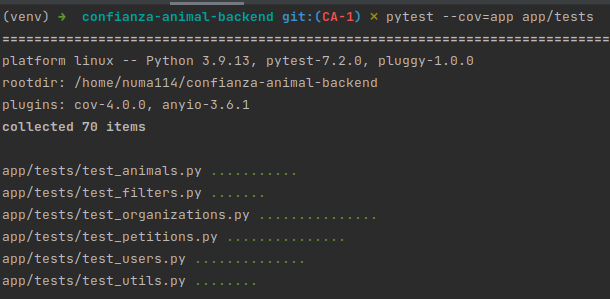
\includegraphics[width=0.8\textwidth]{imgs/coverage2-big.png}
    \caption{Informe de cobertura de los tests de la API}
    \label{fig:coverage2}
\end{figure}

\begin{figure}[H]
    \centering
    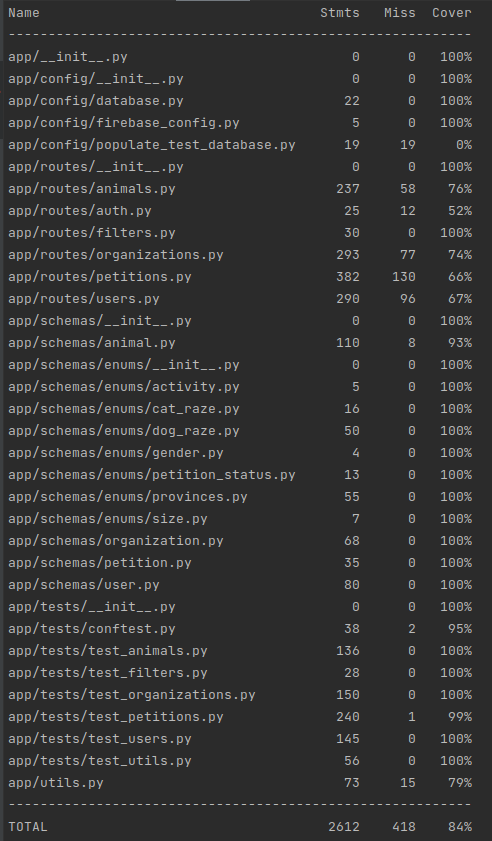
\includegraphics[width=0.8\textwidth]{imgs/coverage1.png}
    \caption{Informe de cobertura de los tests de la API}
    \label{fig:coverage1}
\end{figure}

\newpage

Como se puede observar en las imágenes, la \textbf{cobertura} de los \textit{tests} de la API es del 84\%, la cual se ha obtenido
a partir de la ejecución de 70 \textit{tests} diferentes a lo largo de los diferentes ficheros que se van a explicar
a continuación y que abordan las diferentes casuísticas que se puedan dar en el \textit{endpoint} así como en la base de datos
incluyendo los errores que se puedan producir: \\

\textbf{test\_animals.py}: este fichero contiene los \textit{tests} relacionados con los endpoints de la ruta \textit{/animals} de la API:

\begin{itemize}
    \item \textbf{test\_get\_all\_animals}: este \textit{test} comprueba que se obtienen todos los animales de la base de datos correctamente
    \item \textbf{test\_get\_dog\_by\_id}: este \textit{test} comprueba que se obtiene un perro dado su identificador correctamente.
    \item \textbf{test\_get\_cat\_by\_id}: este \textit{test} comprueba que se obtiene un gato dado su identificador correctamente.
    \item \textbf{test\_get\_dog\_by\_filters}: este \textit{test} comprueba que se obtienen todos los perros que cumplen con los filtros
    especificados por el usuario correctamente (raza, tamaño, etc.) y las diferentes casuísticas que se pueden dar.
    \item \textbf{test\_get\_cat\_by\_filters}: este \textit{test} comprueba que se obtienen todos los gatos que cumplen con los filtros
    especificados por el usuario correctamente (raza, tamaño, etc.) y las diferentes casuísticas que se pueden dar.
    \item \textbf{test\_upload\_dog\_photos}: este \textit{test} comprueba que se suben las fotos de un perro correctamente.
    \item \textbf{test\_upload\_cat\_photos}: este \textit{test} comprueba que se suben las fotos de un gato correctamente.
    \item \textbf{test\_delete\_dog\_photo}: este \textit{test} comprueba que se borra una foto de un perro correctamente.
    \item \textbf{test\_delete\_cat\_photo}: este \textit{test} comprueba que se borra una foto de un gato correctamente.
    \item \textbf{test\_delete\_dog\_by\_id}: este \textit{test} comprueba que se borra un perro dado su identificador correctamente.
    \item \textbf{test\_delete\_cat\_by\_id}: este \textit{test} comprueba que se borra un gato dado su identificador correctamente.
\end{itemize}

\textbf{test\_filters.py}: este fichero contiene los \textit{tests} relacionados con los endpoints de la ruta \textit{/filters} de la API:

\begin{itemize}
    \item \textbf{test\_get\_provinces}: este \textit{test} comprueba que se obtienen todas las provincias correctamente.
    \item \textbf{test\_get\_gender}: este \textit{test} comprueba que se obtienen todos los géneros de los animales correctamente.
    \item \textbf{test\_get\_activity}: este \textit{test} comprueba que se obtienen todas los niveles de actividad de los animales correctamente.
    \item \textbf{test\_get\_size}: este \textit{test} comprueba que se obtienen todos los tamaños de los animales correctamente.
    \item \textbf{test\_get\_cat\_raze}: este \textit{test} comprueba que se obtienen todas las razas de los gatos correctamente.
    \item \textbf{test\_get\_dog\_raze}: este \textit{test} comprueba que se obtienen todas las razas de los perros correctamente.
    \item \textbf{test\_get\_all}: este \textit{test} comprueba que se obtienen todos los filtros anteriores correctamente.
\end{itemize}

\textbf{test\_users.py}: este fichero contiene los \textit{tests} relacionados con los endpoints de la ruta \textit{/users} de la API:

\begin{itemize}
    \item \textbf{test\_user\_register}: este \textit{test} comprueba que se registra un usuario correctamente.
    \item \textbf{test\_login\_user}: este \textit{test} comprueba que se loguea un usuario correctamente.
    \item \textbf{test\_get\_user\_profile}: este \textit{test} comprueba que se obtiene el perfil de un usuario correctamente.
    \item \textbf{test\_user\_favorites}: este \textit{test} comprueba que se obtienen los animales favoritos de un usuario correctamente.
    \item \textbf{test\_check\_if\_animals\_is\_in\_favorites}: este \textit{test} comprueba que se comprueba si un animal está en favoritos de un usuario correctamente.
    \item \textbf{test\_get\_user\_by\_id}: este \textit{test} comprueba que se obtiene un usuario dado su identificador correctamente.
    \item \textbf{test\_envy\_user\_documentation}: este \textit{test} comprueba que se envía la documentación de un usuario correctamente.
    \item \textbf{test\_post\_user\_favorites}: este \textit{test} comprueba que se añade un animal a favoritos de un usuario correctamente.
    \item \textbf{test\_enable\_user}: este \textit{test} comprueba que se habilita un usuario correctamente.
    \item \textbf{test\_disable\_user}: este \textit{test} comprueba que se deshabilita un usuario correctamente.
    \item \textbf{test\_upload\_profile\_photo}: este \textit{test} comprueba que se sube la foto de perfil de un usuario correctamente.
    \item \textbf{test\_update\_user}: este \textit{test} comprueba que se actualiza un usuario correctamente.
    \item \textbf{test\_update\_user\_documentation}: este \textit{test} comprueba que se actualiza la documentación de un usuario correctamente.
    \item \textbf{test\_delete\_favorite}: este \textit{test} comprueba que se borra un animal de favoritos de un usuario correctamente.
\end{itemize}

\textbf{test\_organizations.py}: este fichero contiene los \textit{tests} relacionados con los endpoints de la ruta \textit{/organizations} de la API:

\begin{itemize}
    \item \textbf{test\_organization\_register}: este \textit{test} comprueba que se registra una organización correctamente.
    \item \textbf{test\_login\_organization}: este \textit{test} comprueba que se loguea una organización correctamente.
    \item \textbf{test\_post\_cat}: este \textit{test} comprueba que se añade un gato correctamente a una organización.
    \item \textbf{test\_post\_dog}: este \textit{test} comprueba que se añade un perro correctamente a una organización.
    \item \textbf{test\_get\_organization\_profile}: este \textit{test} comprueba que se obtiene el perfil de una organización correctamente.
    \item \textbf{test\_get\_dogs\_from\_organization}: este \textit{test} comprueba que se obtienen todos los perros de una organización correctamente.
    \item \textbf{test\_get\_cats\_from\_organization}: este \textit{test} comprueba que se obtienen todos los gatos de una organización correctamente.
    \item \textbf{test\_get\_organizations}: este \textit{test} comprueba que se obtienen todas las organizaciones correctamente.
    \item \textbf{test\_get\_organization\_by\_name}: este \textit{test} comprueba que se obtiene una organización dado su nombre correctamente.
    \item \textbf{test\_upload\_profile\_photo\_organization}: este \textit{test} comprueba que se sube la foto de perfil de una organización correctamente.
    \item \textbf{test\_modify\_cat}: este \textit{test} comprueba que se actualizan los datos de un gato correctamente.
    \item \textbf{test\_modify\_dog}: este \textit{test} comprueba que se actualizan los datos de un perro correctamente.
    \item \textbf{test\_enable\_organization}: este \textit{test} comprueba que se habilita una organización correctamente.
    \item \textbf{test\_disable\_organization}: este \textit{test} comprueba que se deshabilita una organización correctamente.
    \item \textbf{test\_update\_organization}: este \textit{test} comprueba que se actualizan los datos de una organización correctamente.
\end{itemize}

\textbf{test\_petitions.py}: este fichero contiene los \textit{tests} relacionados con los endpoints de la ruta \textit{/petitions} de la API:

\begin{itemize}
    \item \textbf{test\_ask\_for\_dog}: este \textit{test} comprueba que la solicitud de un perro se realiza correctamente.
    \item \textbf{test\_ask\_for\_cat}: este \textit{test} comprueba que la solicitud de un gato se realiza correctamente.
    \item \textbf{test\_get\_petitions\_by\_user}: este \textit{test} comprueba que se obtienen todas las solicitudes de un usuario correctamente.
    \item \textbf{test\_get\_petition\_by\_id\_user}: este \textit{test} comprueba que se obtiene una solicitud dado su identificador y el identificador de un usuario correctamente.
    \item \textbf{test\_get\_petitions\_by\_organization}: este \textit{test} comprueba que se obtienen todas las solicitudes de una organización correctamente.
    \item \textbf{test\_reject\_petition\_by\_user}: este \textit{test} comprueba que se rechaza una solicitud por parte de un usuario correctamente.
    \item \textbf{test\_reject\_petition\_by\_organization}: este \textit{test} comprueba que se rechaza una solicitud por parte de una organización correctamente.
    \item \textbf{test\_accept\_petition\_by\_organization}: este \textit{test} comprueba que se acepta una solicitud por parte de una organización correctamente.
    \item \textbf{test\_change\_petition\_visibility\_by\_user}: este \textit{test} comprueba que se cambia la visibilidad de una solicitud por parte de un usuario correctamente.
    \item \textbf{test\_get\_petitions\_visibles\_by\_user}: este \textit{test} comprueba que se obtienen todas las solicitudes visibles de un usuario correctamente.
    \item \textbf{test\_get\_petitions\_invisibles\_by\_user}: este \textit{test} comprueba que se obtienen todas las solicitudes invisibles (archivadas) de un usuario correctamente.
    \item \textbf{test\_update\_state\_petition\_by\_organization}: este \textit{test} comprueba que se actualiza el estado de una solicitud por parte de una organización correctamente.
    \item \textbf{test\_reject\_documentation\_by\_organization}: este \textit{test} comprueba que se rechaza la documentación enviada por un usuario en una solicitud por parte de una organización correctamente.
    \item \textbf{test\_reject\_information\_by\_organization}: este \textit{test} comprueba que se rechaza la información enviada por un usuario en una solicitud por parte de una organización correctamente.
    \item \textbf{test\_accept\_information\_by\_organization}: este \textit{test} comprueba que se acepta la información enviada por un usuario en una solicitud por parte de una organización correctamente.
\end{itemize}

\textbf{test\_utils.py}: este fichero contiene los \textit{tests} relacionados con las funciones auxiliares de la API:

\begin{itemize}
    \item \textbf{test\_exists\_email\_in\_organization}: este \textit{test} comprueba si existe un email en una organización o no.
    \item \textbf{test\_exists\_phone\_in\_organization}: este \textit{test} comprueba si existe un teléfono en una organización o no.
    \item \textbf{test\_exists\_name\_in\_organization}: este \textit{test} comprueba si existe un nombre como nombre de una organización o no.
    \item \textbf{test\_exists\_id\_in\_user}: este \textit{test} comprueba si existe un identificador en un usuario o no.
    \item \textbf{test\_exists\_dog\_in\_animals}: este \textit{test} comprueba si existe un perro en la lista de animales de una organización o no.
    \item \textbf{test\_exists\_cat\_in\_animals}: este \textit{test} comprueba si existe un gato en la lista de animales de una organización o no.
    \item \textbf{test\_get\_dog\_or\_cat\_by\_filters}: este \textit{test} comprueba que se obtienen los perros o gatos que cumplen los filtros correctamente.
    \item \textbf{test\_generate\_uuid}: este \textit{test} comprueba que se genera un identificador único correctamente.
\end{itemize}

A parte de todos los \textit{tests} mencionados anteriormente, se han realizado una serie de \textit{fixtures} (datos de prueba) para poder realizar los \textit{tests} de forma correcta.
Estas \textit{fixtures} se encuentran en el fichero \textbf{conftest.py} y son para poder acceder a los \textit{endpoints} que requieren
de autenticación, por tanto existe una \textit{fixture} para la autenticación de un usuario y otra para la autenticación de una organización.
Se identifican por medio de los \textit{decorators} \@pytest.fixture y se usan directamente en los \textit{tests} que las requieren pasándolas como parámetro. \\

Un ejemplo de \textbf{test de integración} sería el \textit{test\_accept\_petition\_by\_organization} ya que
para poder realizarlo se necesita comprobar toda la funcionalidad asociada a la aceptación de una solicitud por parte de una organización:

\begin{enumerate}
    \item Se crea una organización y un usuario.
    \item Se crea una solicitud por parte del usuario a la organización.
    \item La organización actualiza el estado de la solicitud a \textit{Información pendiente de revisión}.
    \item La organización comprueba que la información aportada es correcta, acepta la información enviada por el usuario y actualiza el estado de la solicitud a \textit{Pendiente de documentación}.
    \item El usuario envía la documentación requerida por la organización.
    \item La organización acepta la documentación enviada por el usuario y actualiza el estado de la solicitud a \textit{Aceptada}.
\end{enumerate}

Es por ello que para realizar este \textit{test} es necesario completar todo el flujo de la petición (ver completo en la figura:~\ref{fig:flujo_peticion}) y comprobar que
la funcionalidad asociada a cada paso se realiza correctamente teniendo en cuenta también los posibles casos que se pueden
dar durante el proceso, como por ejemplo que la organización rechace la información enviada por el usuario y actualice el estado de la solicitud a \textit{Información rechazada}
y que el usuario envíe de nuevo la información requerida por la organización. \\

En cuanto a los tests de la aplicación web, por cada componente y servicio existe un fichero de \textit{tests} asociado bajo
la extensión \textbf{.spec.ts}. Dado que el proyecto está enfocado en el desarrollo de la API, no se han realizado demasiados
\textit{tests} en la aplicación web, pero se han realizado algunos para comprobar que los componentes y servicios funcionan correctamente. \\

Un ejemplo de \textit{test} muy básico de un componente en el que se comprueba que se crea correctamente sería el siguiente:

\begin{lstlisting}
  describe('DogViewComponent', () => {
      let component: DogViewComponent;
      let fixture: ComponentFixture<DogViewComponent>;

      beforeEach(async () => {
        await TestBed.configureTestingModule({
          imports: [
            DogViewComponent,
            HttpClientTestingModule,
            ToastrModule.forRoot(),
            StoreModule.forRoot({}),
          ],
        }).compileComponents();

        fixture = TestBed.createComponent(DogViewComponent);
        component = fixture.componentInstance;
        fixture.detectChanges();
      });

      it('should create', () => {
        expect(component).toBeTruthy();
      });
  });
\end{lstlisting}



\subsection{Sprints 9-11}\label{subsec:sprints-9-11}

En los tres últimos \textit{sprints} se han llevado a cabo las tareas que han permitido el cierre del proyecto. En concreto, se ha
llevado a cabo la finalización de los \textit{tests} pendientes, el cierre final de tareas y la finalización
y revisión de la página web, del funcionamiento de la API y de la documentación del proyecto.

\subsubsection{Documentación de la API}\label{subsubsec:documentacion-api}

La documentación de la API se ha realizado utilizando \href{https://www.swagger.io/}{Swagger}. Swagger es una herramienta que permite
documentar APIs de forma sencilla y que proporciona una interfaz gráfica para poder probar las APIs. Esta documentación
se encuentra de forma pública en el siguiente enlace: \href{https://confianza-animal-backend.onrender.com/docs}{Confianza Animal Docs}. \\

Todos los endpoints en la documentación cuentan con un ejemplo de petición: (ver en siguiente página)

\begin{figure}[H]
    \centering
    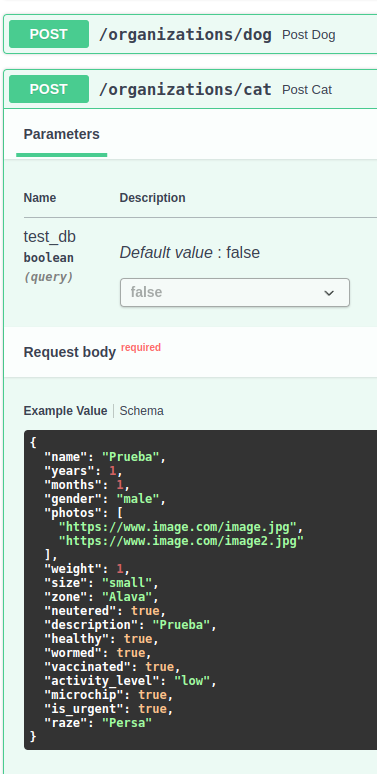
\includegraphics[width=0.5\textwidth]{imgs/swagger1.png}
    \caption{Ejemplo de petición en la documentación}
    \label{fig:endpoint-example}
\end{figure}

\newpage

Y un ejemplo de respuesta y de error: \\

\begin{figure}[H]
    \centering
    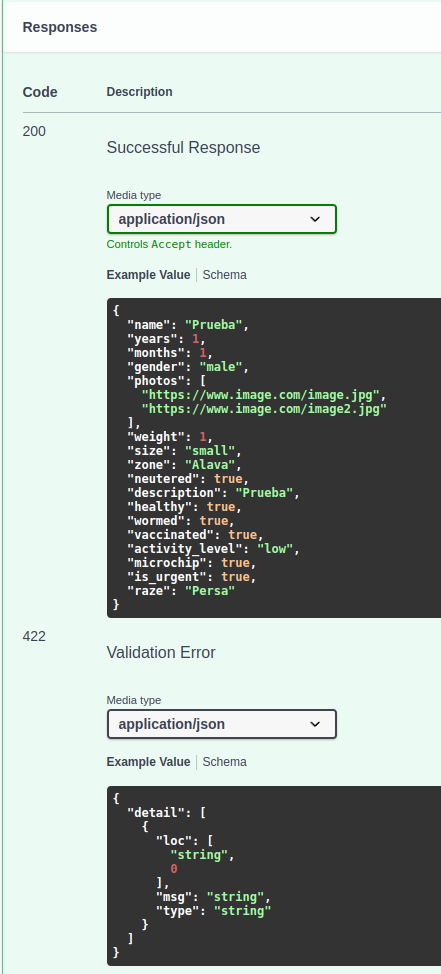
\includegraphics[width=0.5\textwidth]{imgs/swagger2.png}
    \caption{Ejemplo de respuesta y error en la documentación}
    \label{fig:endpoint-example-2}
\end{figure}

De esta forma, ayuda a los desarrolladores a entender cómo funciona la API y a realizar peticiones de forma correcta sin
necesidad de tener que leer el código. También permite a usuarios con menos conocimientos técnicos tener la oportunidad
de utilizar la API ya que la interfaz es muy intuitiva.


\section{Despliegue de la página web}\label{sec:despliegue-de-la-pagina-web}

Para el despliegue de la página web se ha utilizado \textit{Firebase Hosting}, un servicio de hosting web que permite
desplegar aplicaciones web estáticas de forma sencilla y rápida. \textit{Firebase Hosting} ofrece un plan gratuito que
incluye 10 GB de almacenamiento y 10 GB de transferencia de datos al mes, más que suficiente para el desarrollo de este
proyecto en fase de pruebas. \\

Tal y como se mencionó en la sección:~\ref{sec:eleccion-de-herramientas-y-tecnologias}, gracias a que la página web
está desarrollada con \textbf{Angular} y esta ser un framework de \textbf{Google}, la integración con \textit{Firebase}
es muy sencilla y no presenta problemas de compatibilidad a la hora de llevar a cabo el despliegue para el cual
se han seguido los siguientes pasos:

\begin{enumerate}
    \item Instalar \textit{Firebase CLI} por medio de \textit{npm} con el comando \textit{npm install -g firebase-tools}.
    \item Iniciar sesión en \textit{Firebase} con el comando \textit{firebase login}.
    \item Inicializar el proyecto con el comando \textit{firebase init}.
    \item Seleccionar la opción \textit{Hosting} y el proyecto de \textit{Firebase} que se quiere desplegar.
    \item Seleccionar la carpeta que contiene el código de la página web.
    \item Ejecutar el comando \textit{firebase deploy} para desplegar la página web.
\end{enumerate}

Es por ello que de esta forma, cada vez que se realice un cambio en el código de la página web se puede desplegar de forma automática
con el comando \textit{firebase deploy}. Otra ventaja que ofrece esta herramienta es que permite la creación de un dominio personalizado
para la página web y la configuración de certificados \textit{TSL} gratuitos para que la página web se pueda acceder por medio de
\textit{HTTPS} con el dominio personalizado. De forma predeterminada, \textit{Firebase Hosting} ofrece un dominio gratuito
con el siguiente formato: \textit{<nombre-proyecto>.web.app} que se accede por medio de \textit{HTTPS}. En este caso, la ruta
de acceso a la página web es: \url{https://confianza-animal.web.app}.

En la siguiente figura se puede ver el resultado de acceder al enlace de la página web: \\

\begin{figure}[H]
    \centering
    
\includegraphics[width=0.9\textwidth]{imgs/despliegue-web.png}
    \caption{Despliegue de la página web en Firebase Hosting}
    \label{fig:firebase-hosting}
\end{figure}

\section{Despliegue de la API}\label{sec:despliegue-de-la-api}

Para el despliegue de la API y su documentación se ha utilizado \textbf{Render}, un servicio de hosting con certificados \textit{TSL}
gratuitos, una \textit{CDN} global, protección \textit{DDoS}, redes privadas y despliegues automáticos desde \textit{GitHub}.
Los detalles de seguridad del proyecto así como los protocolos que se utilizan para la comunicación entre el cliente y el servidor
se pueden consultar en profundidad en la sección de seguridad:~\ref{sec:seguridad}. \\

El motivo principal por el que se ha escogido Render para el despliegue de la API es por su facilidad de uso y por su
integración con \textit{GitHub}. Render permite desplegar la API de forma automática cada vez que se realiza un cambio
en el repositorio de \textit{GitHub} y permite la creación de un dominio personalizado para la API. \\

Otro tema que ha decidido la elección de esta herramienta ha sido el precio. Render ofrece un plan gratuito que incluye
750 horas de uso, 100 GB de ancho de banda y 500 minutos de \textit{build} que se renuevan cada mes. Este plan ha sido
más que suficiente para el desarrollo del proyecto pero en caso de que el proyecto se siguiera desarrollando, Render
ofrece planes de pago que permiten escalar los recursos de forma sencilla y sin necesidad de preocuparse por la
gestión de los servidores. \\

\begin{figure}[H]
    \centering
    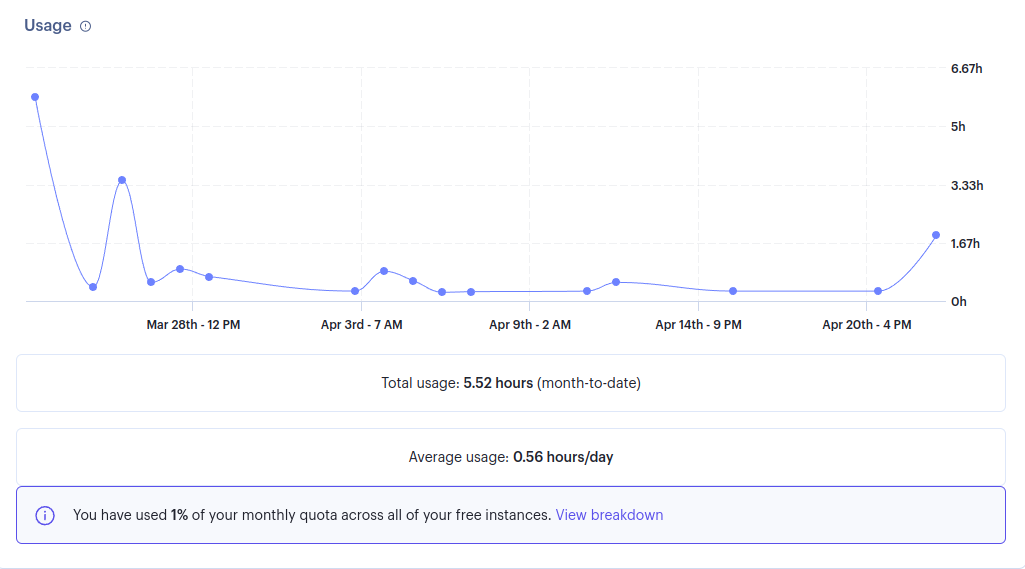
\includegraphics[width=0.9\textwidth]{imgs/usage.png}
    \caption{Uso total de la API}
    \label{fig:usage-render}
\end{figure}

\begin{figure}[H]
    \centering
    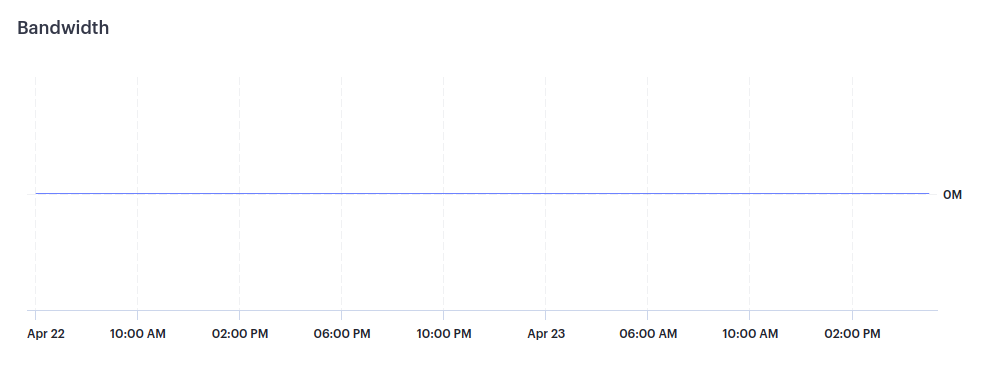
\includegraphics[width=0.9\textwidth]{imgs/bandwidth.png}
    \caption{Ancho de banda total de la API}
    \label{fig:bandwidth-render}
\end{figure}

Los pasos que se han seguido para realizar el despliegue han sido los siguientes:

\begin{enumerate}
    \item Vincular la cuenta de \textit{GitHub} con Render.
    \item Crear un nuevo servicio que se conecte a nuestro repositorio deseado.
    \item Crear un \textit{environment} (entorno) para el servicio. En este caso se han añadido las variables de entorno
    correspondientes a la base de datos y a los servicios de Firebase y tres ficheros que almacenan claves privadas:
    un json con las claves de la base de datos de producción, un json con las claves de la base de datos de test
    y el fichero \textit{.env} con todas las variables de entorno que se utilizan en el proyecto.
    \item Instalar los paquetes necesarios para el despliegue de la API. En este caso al ser un proyecto con \textit{Python}
    se ha utilizado el fichero \textit{requirements.txt} el cual por medio del comando \textit{pip install -r requirements.txt}
    se incluyen paquetes como \textit{pytest}, \textit{firebase}, \textit{FastAPI}, \textit{uvicorn}, etc.
    \item Para lanzar la API se utiliza el comando \textit{uvicorn main:app --host 0.0.0.0 --port 10000} que permite
    correr el servidor de \textit{FastAPI} en el puerto 10000 (puerto por defecto de Render).
    \item Se selecciona la rama de nuestro repositorio se quiere desplegar (\textit{main} en este caso) y la rama de
    despliegue automático cada vez que se realice un \textit{push} (cambio en el código).
\end{enumerate}

Un aspecto importante a tener en cuenta es que para el despliegue de la API se lanza el comando \textit{pytest} para
ejecutar todos los tests antes de hacer el despliegue. Esto permite asegurarnos de que nuestro código funciona correctamente
y que la funcionalidad cumple los \textit{tests} realizados en el proyecto antes de sacar una nueva versión de forma pública.

\begin{figure}[H]
    \centering
    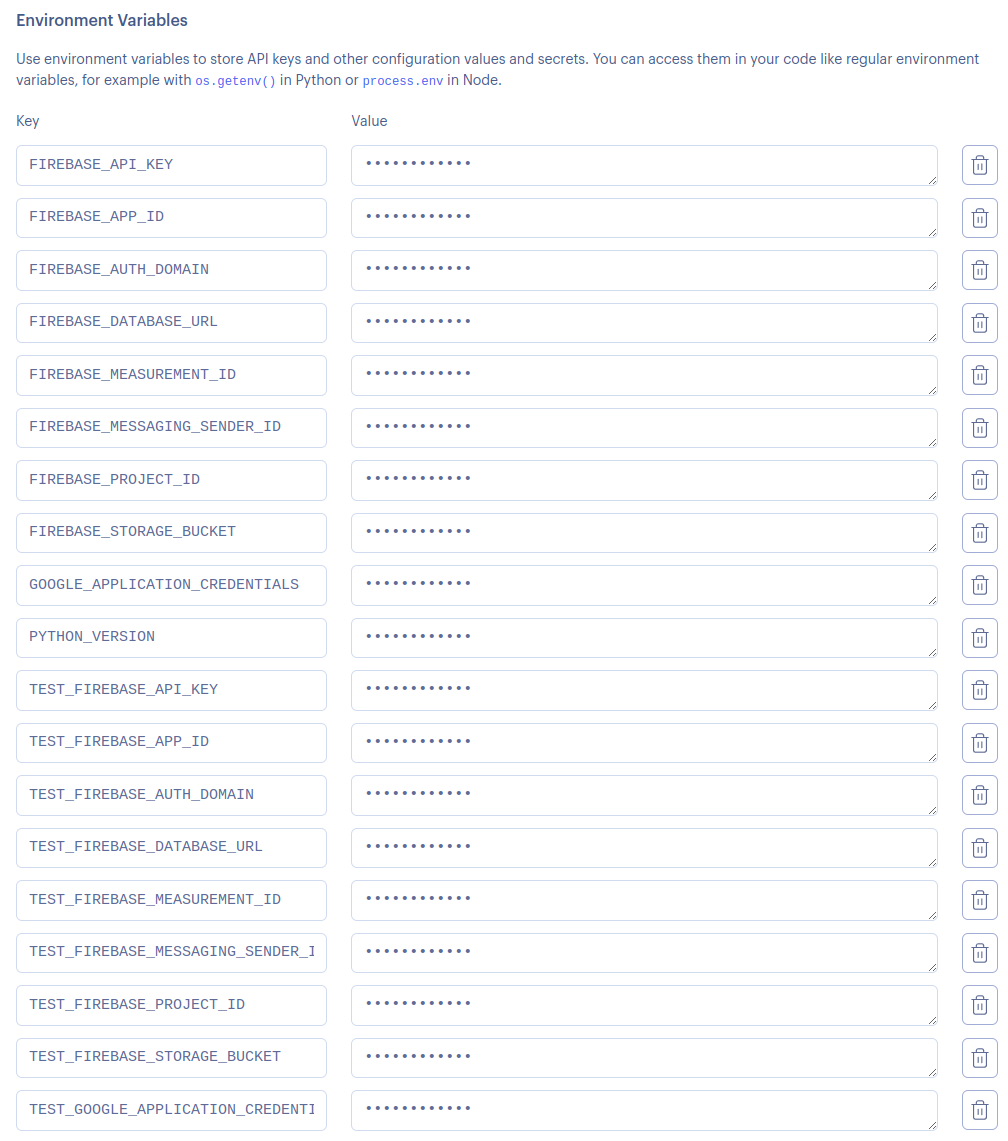
\includegraphics[width=0.8\textwidth]{imgs/env-variables.png}
    \caption{Variables de entorno}
    \label{fig:environment-variables}
\end{figure}

\begin{figure}[H]
    \centering
    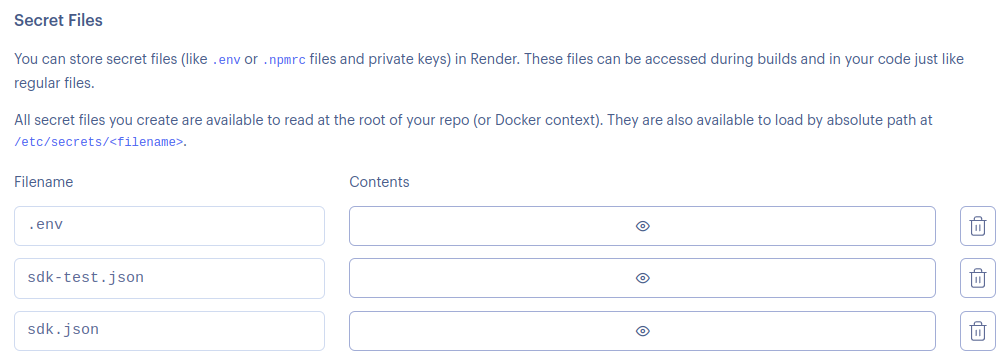
\includegraphics[width=0.8\textwidth]{imgs/secret-files.png}
    \caption{Ficheros secretos}
    \label{fig:secret-files}
\end{figure}

\newpage